\section{Methodology}
    % Über Bau des Spektrometers erzählen
    % Formeln erklären
    % Argumentieren warum wir grating constant vom internet nehmen

    To build the spectrometer, cardboard, tape, two razor blades, a CD and a camera (ideally wide angle) is needed.
    The less reflective the cardboard is, the better the results are going to be.
    Build a tube with the cardboard and attach the two razor blades to one end, leaving just a small slit of about 0.2 mm for light to enter.
    Remove the reflective foil off the CD using a cutter and tape and cut out a piece of the transparent part of the size of the cardboard tube.
    tape it to the open end of the tube.
    Now attach the camera to the same side.
    make sure no light enters the apparatus except through the slit.

    If held in the direction of a light source, a diffraction pattern, showing the spectrum of the different wavelengths, is visible on the camera.
    The formula relating the distance of the maxima of different orders to the wavelength of the light entering the spectrometer is given in equation~\eqref{eq_interference}.

    \begin{align}
        p \lambda = g \sin(\phi) \label{eq_interference}
    \end{align}

    $p$ is an integer called the order number. For the first visible maximum, $p$ is equal to $1$, for the second maximum $p = 2$ and so on.
    $\lambda$ is the wavelength of the light.
    The grating constant $g$ is dependent on the distance between the slits in the grating.
    Hence this constant is not the same for different kinds of CDs or DVDs.
    the last variable is the angle $\phi$ in the triangle of the maximum of zero and $p^{th}$ order and the spot where the light passes through the grating, measured at the grating.
    Trigonometry gives the relation $\tan(\phi) = \frac{x_p}{d}$, which is visible in the figure~\ref{fig_phi}.

    \begin{figure}[H]
        \centering
        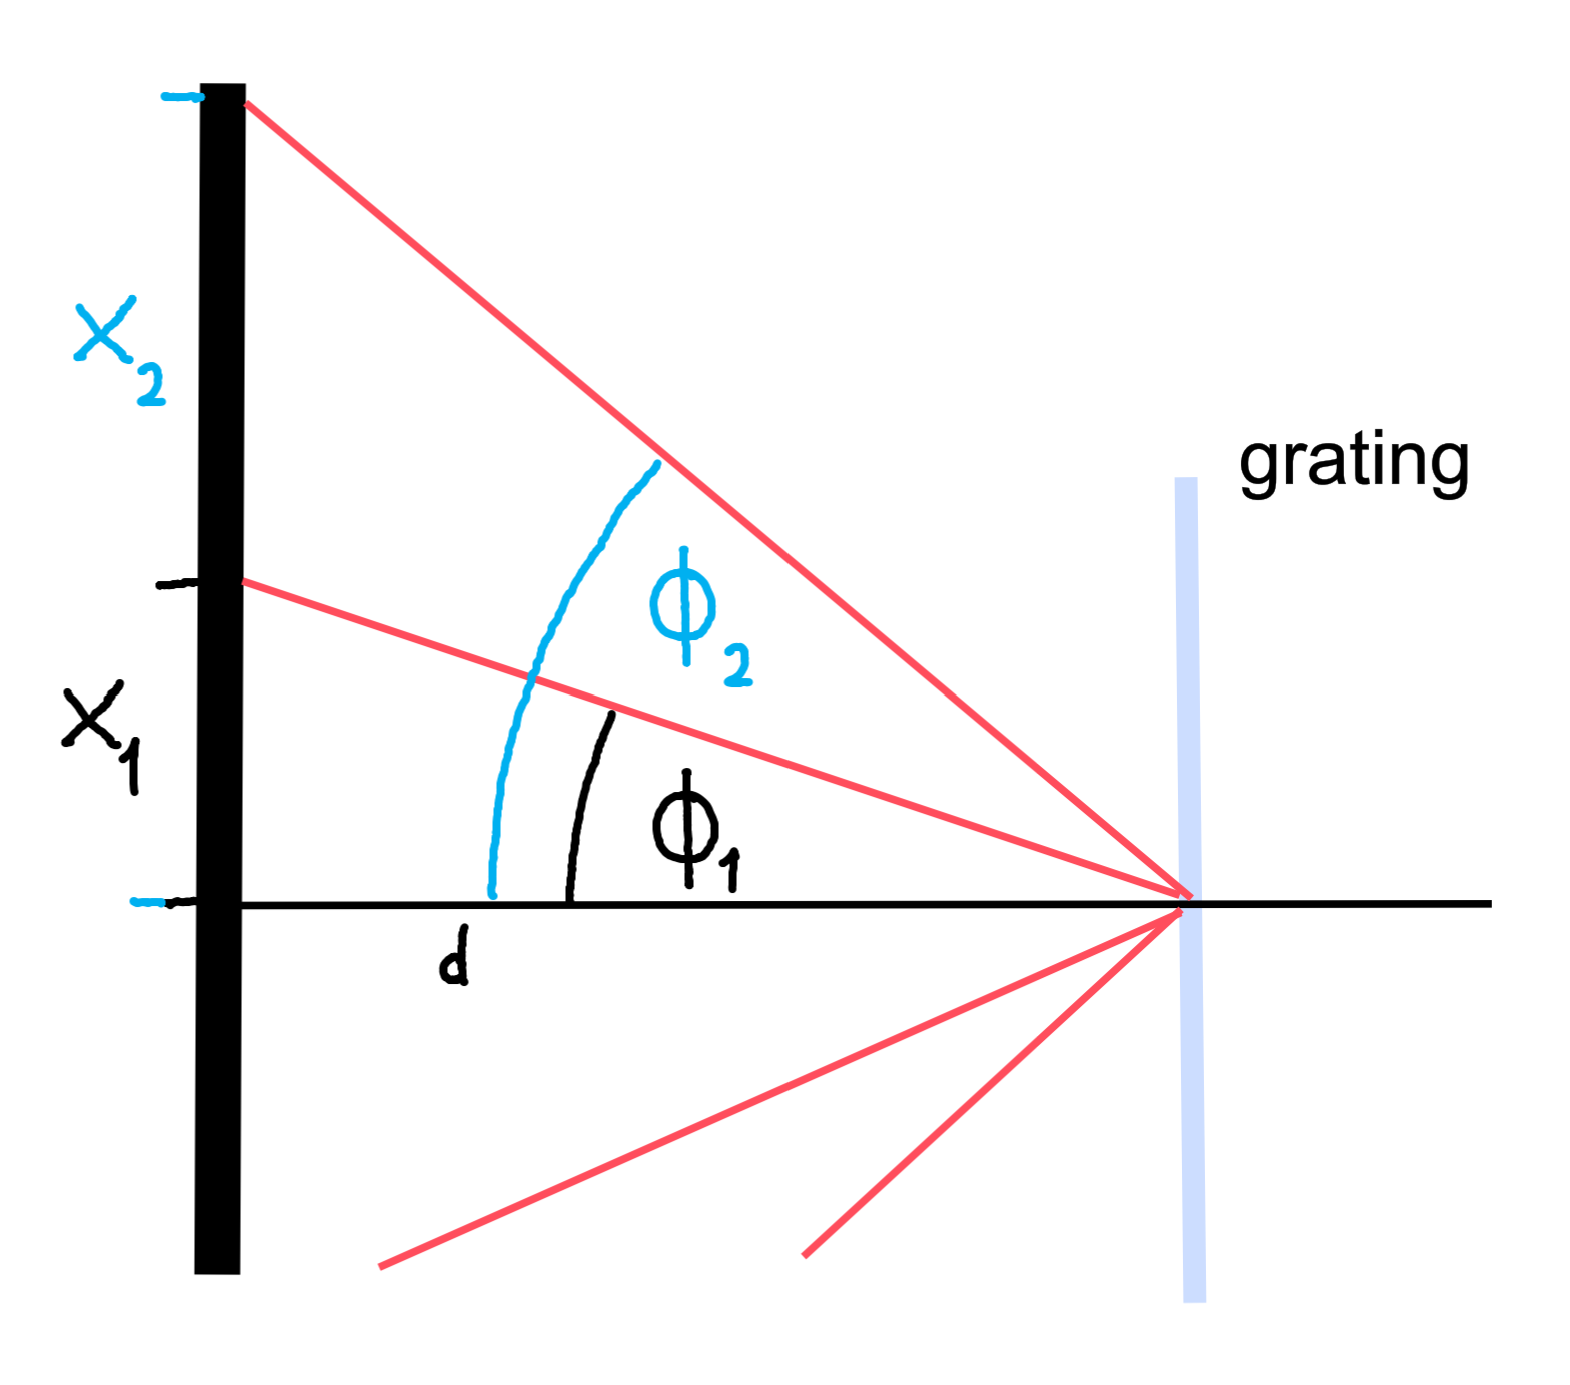
\includegraphics[scale = 0.7]{src/images/angle_phi.png}
        \caption{Visualization of the location of the angle $\phi$ referred to in equation~\eqref{eq_interference}.
        The first and second maximum of one certain wavelength is shown, so monochromatic light would be needed to reproduce this hypothetical situation.}
        \label{fig_phi}
    \end{figure}

    In our test case, we assumed a grating constant $g = 1.514 \mu m$ \cite{src_grating_constant} as we did not have a monochromatic light source at hand to determine the grating constant of our CD.
    Next, we calculated the distance between the CD and the camera to calibrate our spectrometer using a first measurement and by choosing a certain colour and its corresponding wavelength.


    We have multiple goals in this experiment series:
    \begin{enumerate}
        \item The calibration of the pressure sensor and its corresponding pressures.
        \item Determination of the absolute zero point of temperature.
        \item Determination of the temperature of liquid nitrogen.
    \end{enumerate}
    We will achieve these results by making use of the linearly corresponding properties of ideal gases with the help of the apparatus shown in Fig.~\ref{fig_setup}.

    

    Starting with the calibration of the voltmeter, the voltages at room pressure and when a vacuum pump is connected are noted and compared to the actual pressure in the room and the pressure, the pump is able to maintain.
    Hereafter, the glass bulb is evacuated and filled with helium, the reason being that the properties of helium are closer to ideal gases than air.
    Moreover, the oxygen from the air would liquefy when cooled down to the temperature of liquid nitrogen (which would happen in the third step of the experiment series) and liquids do not act according to the ideal gas equation.

    In the next step, the helium-filled glass bulb is heated to the boiling point of water using steam while leaving the apparatus open so that excess helium can escape.
    We chose the temperature of boiling water as the value can easily be calculated using ambient temperature and pressure as well as tabulated data.
    The gas will only expand in this step and hence no air will get into the glass bulb.
    As soon as the helium has reached the desired temperature, the voltage is taken and the system is closed back up at opening 6. (see Fig.~\ref{fig_setup})
    From now on, the closed system can be used just like a thermometer when calculating the temperature at its corresponding voltage.
    
    To create a linear relation of pressure and temperature in the bulb, a second measurement is needed.
    The temperature at the freezing point of water is also known, so this is the second point used in our case.
    The Helium filled bulb is cooled in an ice bath and the voltage is taken.
    To calculate the absolute zero point of temperature, we have to pay respect to the expansion of the glass bulb with increasing temperature.
    Please refer to section~\ref{sec_results} for the calculation.

    As mentioned before, the closed system acts like a thermometer.
    Therefore, we can cool down the helium filled bulb using liquid nitrogen, read off the voltage and calculate the corresponding temperature of liquid nitrogen.
    In this step, the expansion of the glass bulb must be taken into account as well.

    The error sources in this experiment can be classified:
    \begin{itemize}
        \item In our analysis, it is assumed that the temperature in the room stays the same during the whole process.
        Needless to say that this does not have to be the case: small fluctuations happen naturally.
        As a result, corrupted data could occur during the calibration of the sensor.
        Furthermore, the temperature was read off an analog thermometer leading to an uncertainty caused by the limits of the human eye.
        \item Next to the temperature, the pressure does also fluctuate over time.
        The boiling point of water depends on the pressure.
        Hence, when heating the helium to the boiling point of water, a deviation in the temperature used in calculations below and the real temperature could exist.
        As with temperature, the pressure was also read off an analog measurement device and this value could slightly differ from the real pressure.
        \item The manufacturer of the sensor has defined a certain nonlinearity in the conversion of pressure to its corresponding voltage.
        \item The pump does not create an absolute vacuum and small amounts of air could stay in the glass bulb.
        This would have the biggest impact on the temperature measurement of liquid nitrogen as parts of the air would liquify and the linearity resulting from the ideal gas law eq.~\ref{eq_igl} would not be maintained.
        \item When heating and cooling the gas in the bulb, the glass itself could need more time to evenly distribute the temperature resulting in an uneven change in the gas volume, therefore changing the pressure.
        This would affect the difference between the linear approach and the exact calculation of $t_0$ and $t_{LN2}$.
    \end{itemize}
